\documentclass{beamer}
%\documentclass[handout]{beamer}

\mode<presentation>
{
  %\usetheme{Warsaw}
  \usetheme{Frankfurt}
  %\usetheme[subsection=false]{Dresden}
  \useoutertheme[subsection=false]{miniframes}
  \usecolortheme{beaver}
  \useinnertheme{circles}

  \setbeamercovered{highly dynamic}
  \setbeamertemplate{navigation symbols}{}
}

\usepackage[english]{babel}
\usepackage[utf8]{inputenc}
\usepackage{color}

\usepackage{lmodern}
\usepackage[T1]{fontenc}

\title
{Mutualism in the face of parasitism: a population dynamics approach}

\author[]
{Renato Mendes Coutinho\inst{1} \and Yazmín Zurita-Guti\'errez
\inst{2} \\ \and Edgar Zanella Alvarenga\inst{3}}

\institute[IFT]
{
  \inst{1}
  Institute for Theoretical Physics\\
  S\~ao Paulo State University\\
  \texttt{renato.coutinho@gmail.com}
  \and
  \inst{2}
  Centre d'Ecologie Fonctienelle et Evolutive \\
  Montpellier - France \\
  \texttt{ravenzurapiti@ciencias.unam.mx}
  \and
  \inst{3}
  Bioinformatics Program at IME - University of S\~ao Paulo \\
  \texttt{e@vaz.io}
}

\date[DS Bio 2014] % (optional, should be abbreviation of conference name)
{
  \vspace{0.2cm} Minischool on Dynamical Systems in Biology}

% If you wish to uncover everything in a step-wise fashion, uncomment
% the following command: 
%\beamerdefaultoverlayspecification{<+->}

\begin{document}

\begin{frame}
  \titlepage
\end{frame}

\begin{frame}{Outline}{}
  \tableofcontents[pausesections]
\end{frame}

\section{Mutualism: service relationships}

\begin{frame}{Mutualism: service-resource relationships}
\begin{columns}
    \column{.3\textwidth}
        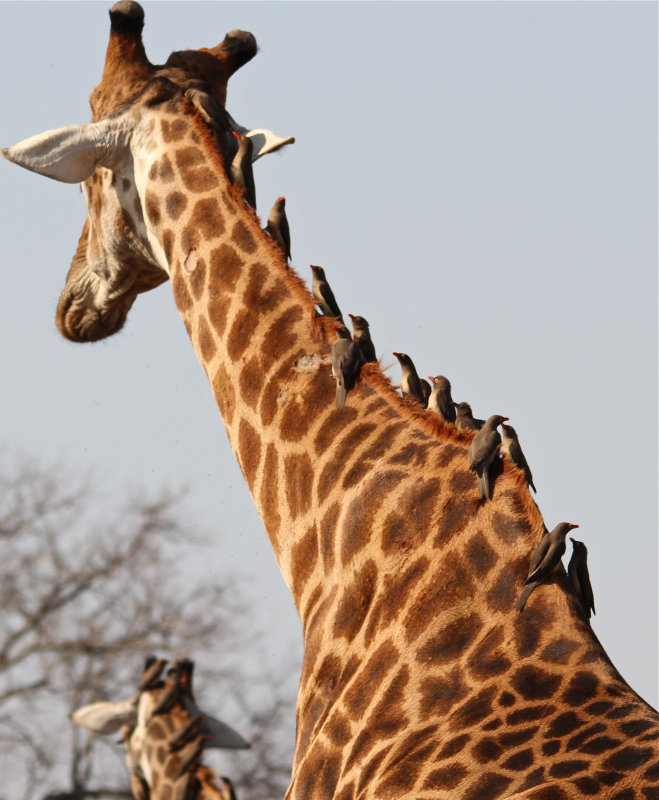
\includegraphics[width=.7\textheight]{birdeatgiraffe.jpg} \\
    \column[t]{.5\textwidth}
        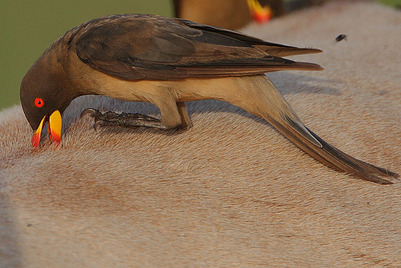
\includegraphics[width=.9\textwidth]{limpiando.jpg}
        \vfill
\end{columns}
\end{frame}

\begin{frame}{A few examples}
\begin{columns}
    \column{.6\textwidth}
        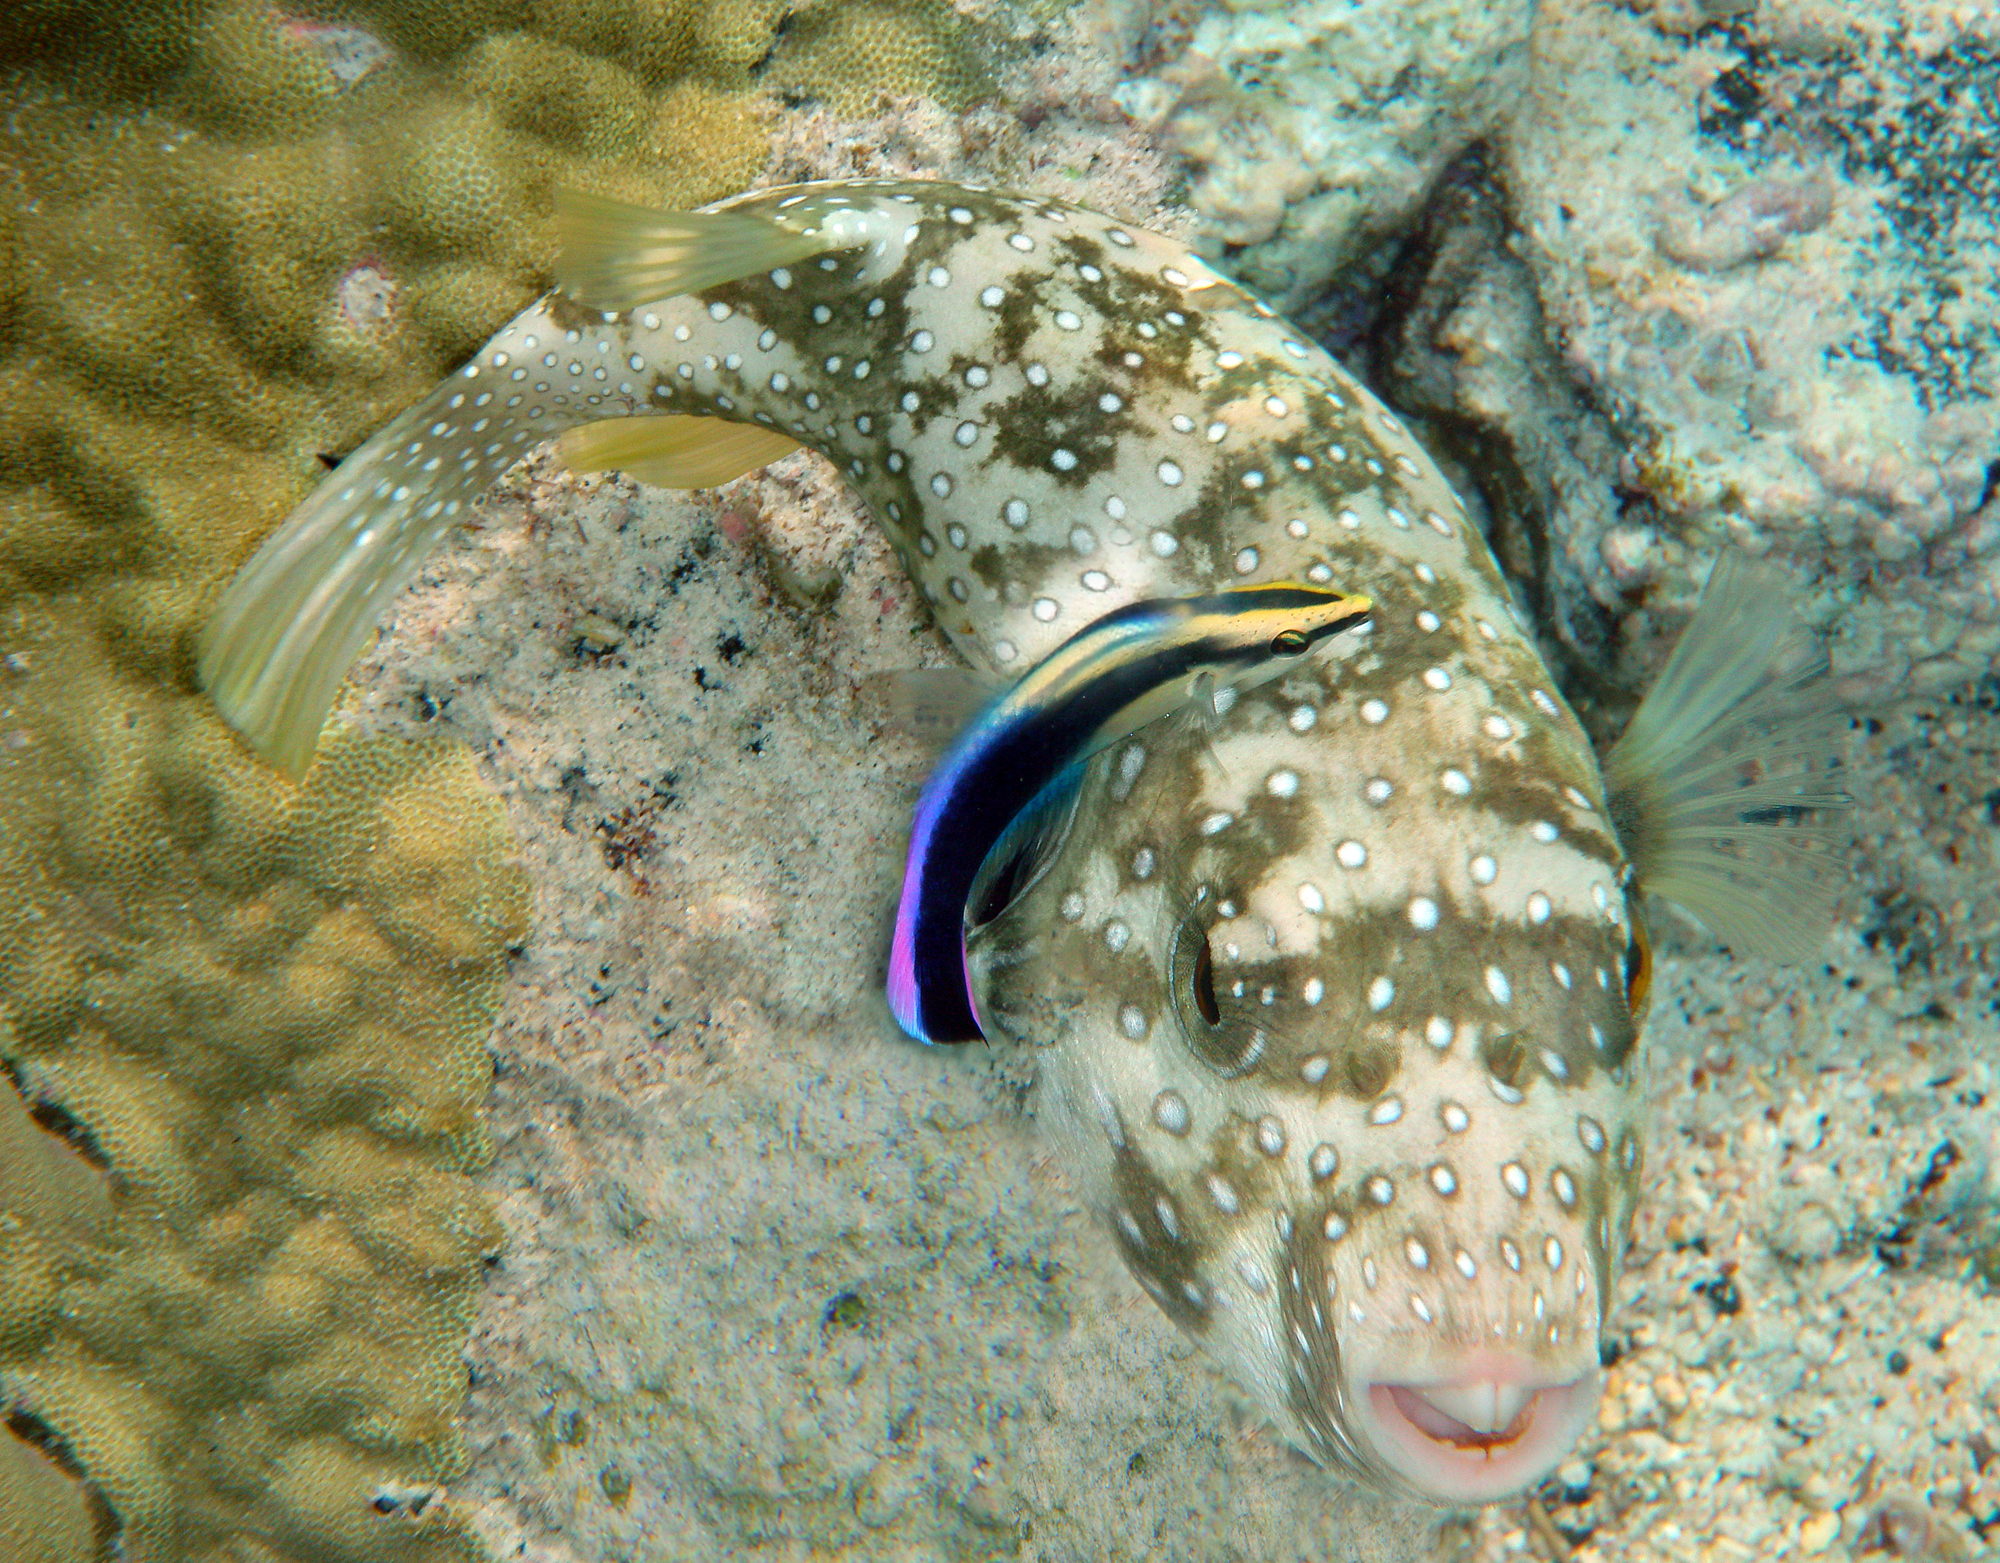
\includegraphics[width=1\textwidth]{fishcoral.jpg} \\
    \column[t]{.5\textwidth}
        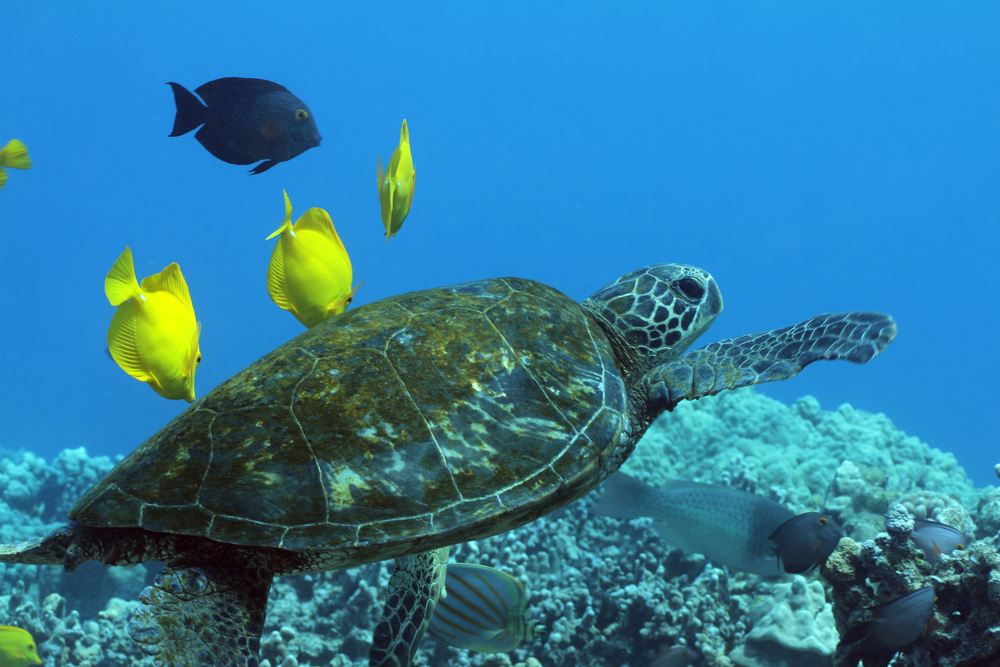
\includegraphics[width=1\textwidth]{turtle.jpg}

\end{columns}
\end{frame}

\begin{frame}{Mutualism \emph{vs.} Parasitism}
        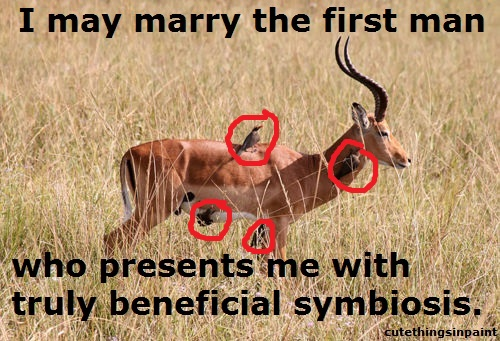
\includegraphics[width=1\textwidth]{marryme.jpg} \\
\end{frame}

\begin{frame}{Mutualism \emph{vs.} parasitism}
    \begin{block}{
        How can mutualism be maintained if parasitism seems to be advantageous?}
\begin{itemize}
    \item We investigated this question developing a model for the population
        dynamics of a cleaner-client relationship.
    \item We chose a few specific assumptions, but the idea was to assess
        general qualitative ideas of why and how this kind of system keeps its
        mutualistic character.
\end{itemize}
\end{block}
\end{frame}


\section{Model formulation}

\begin{frame}{Model formulation and assumptions}
    We formulate a model for the growth, in continuous time, of the
    populations of clients ($H$ for hosts), cleaners ($M$ for mutualists) and
    their food ($D$ for detritus).
            \pause
    \begin{itemize}
        \item Hosts population grow logistically;
            \pause
        \item detritus reduce the growth of hosts.
            \pause
        \item Cleaners feed on detritus.
            \pause
        \item Hosts can avoid mutualists, either by avoiding them or scraping
            them off.
            \pause
        \item The amount of detritus increases with the abundance of hosts.
            \pause
        \item Cleaners may also be harmful to the hosts, for instance by
            feeding on them.
    \end{itemize}
\end{frame}

\begin{frame}{The model}
\begin{align*}
    \frac{dH}{dt} &= \overbrace{H \rho(H)}^{\text{host growth}} \pause
        - \overbrace{\alpha DH}^\text{effect of detritus} \pause
        - \overbrace{\frac{(1-q)H}{1+qahD + (1-q)a h_P H}
    aM}^\text{parasitism} \\[3ex]
    \pause
    \frac{dM}{dt} &= \frac{\overbrace{qD}^\text{feeding on detritus} \pause +
    \overbrace{(1-q)H}^\text{feeding on the host}}{1+qahD + (1-q)a h_P H} aM \pause 
    \\ & \qquad {}
    - \overbrace{\mu M}^\text{natural mortality}\pause
    + \overbrace{\frac{\beta M}{D}}^\text{avoidance by the host}\\[2ex]
    \pause
    \frac{dD}{dt} &= \underbrace{i_D H}_\text{detritus accumulation} \pause -
    \underbrace{sD}_\text{detritus degradation} \pause - \underbrace{\frac{aqDM}{1+qahD + (1-q)a h_P H}}_\text{feeding on detritus}
\end{align*}
\end{frame}


\section{Questions and sort of answers}

\begin{frame}{Questions to the model}
The model includes two key parameters, related to the species' behavior:
\pause
    \begin{itemize}
        \item $q$ is the preference of cleaner for feeding on detritus
            instead of hosts, so "benign" cleaners have $q=1$. \pause
        \item $\beta$ represents the avoidance of cleaners by hosts \pause
    \end{itemize}
    These two behavioral aspects could evolve in response to each other.

\end{frame}
\begin{frame}{Questions to the model}
    Our model allows us to pose some interesting questions:
\pause
    \begin{itemize}
        \item Under which conditions there is coexistence of hosts and
            mutualists?
\pause
        \item Is there an optimal preference $q$ for mutualists?
\pause
        \item Is there an optimal cleaning effort $\beta$ for hosts?
\pause
        \item Is there an evolutionary stable strategy (ESS) when both $q$ and $\beta$ are allowed to change?
    \end{itemize}

\end{frame}

\begin{frame}{How to address the questions}

\begin{align*}
    \frac{dH}{dt} &= H (\rho(H) - \alpha D) - \frac{(1-q)H}{1+qahD + (1-q)a h_P H} aM 
        \\&\qquad \textcolor{purple}{- \frac{(1-q')H}{1+q'ahD + (1-q')a h_P H} aM'} \\[2ex]
    \frac{dM}{dt} &= \frac{qD + (1-q)H}{1+qahD + (1-q)a h_P H} aM - \left(\mu + \frac{\beta}{D}\right) M \\[2ex]
    \frac{dD}{dt} &= i_D H- sD - \frac{qD}{1+qahD + (1-q)a h_P H} aM 
         \\&\qquad   \textcolor{purple}{- \frac{q'D}{1+q'ahD + (1-q')a h_P H} aM'} \\[2ex]
    \textcolor{purple}{\frac{dM'}{dt} }&\textcolor{purple}{= \frac{q'D + (1-q')H}{1+q'ahD + (1-q')a h_P H} aM' - \left(\mu +  \frac{\beta}{D}\right) M'}
\end{align*}

\end{frame}

\begin{frame}{How to address the questions}

    At the equilibrium $$\frac{dH}{dt} = \frac{dM}{dt} = \frac{dD}{dt} = 0$$

We analysed if the mutant $M'$ is able to invade this equilibrium, by
verifying if $$\frac{dM'}{dt} > 0$$ with a initial $M'$ close to zero, and $q' \neq q$
(all other parameters are the same).  

\end{frame}

\begin{frame}{A few answers}
    \begin{block}{Under which conditions there is coexistence of hosts and
        ``benign'' mutualists?}
        Analysing the coexistence fixed point, some conditions have to be
        satisfied to ensure that it exists (ie. it is positive):
$$\begin{aligned}
    \mu &< \frac{1}{h} &&\Rightarrow \text{mortality smaller than maximum
    feeding rate}\\
    \frac{\alpha}{r} &< 1 -s &&\Rightarrow \text{not everything is easy to
    interpret!}\\
    r &> \frac{\alpha i_D}{s} &&\Rightarrow \text{host growth rate greater than
    detritus effect}
   \end{aligned}$$
    \end{block}

\end{frame}

\begin{frame}{Model outcomes: equilibrium (without mutant)}
    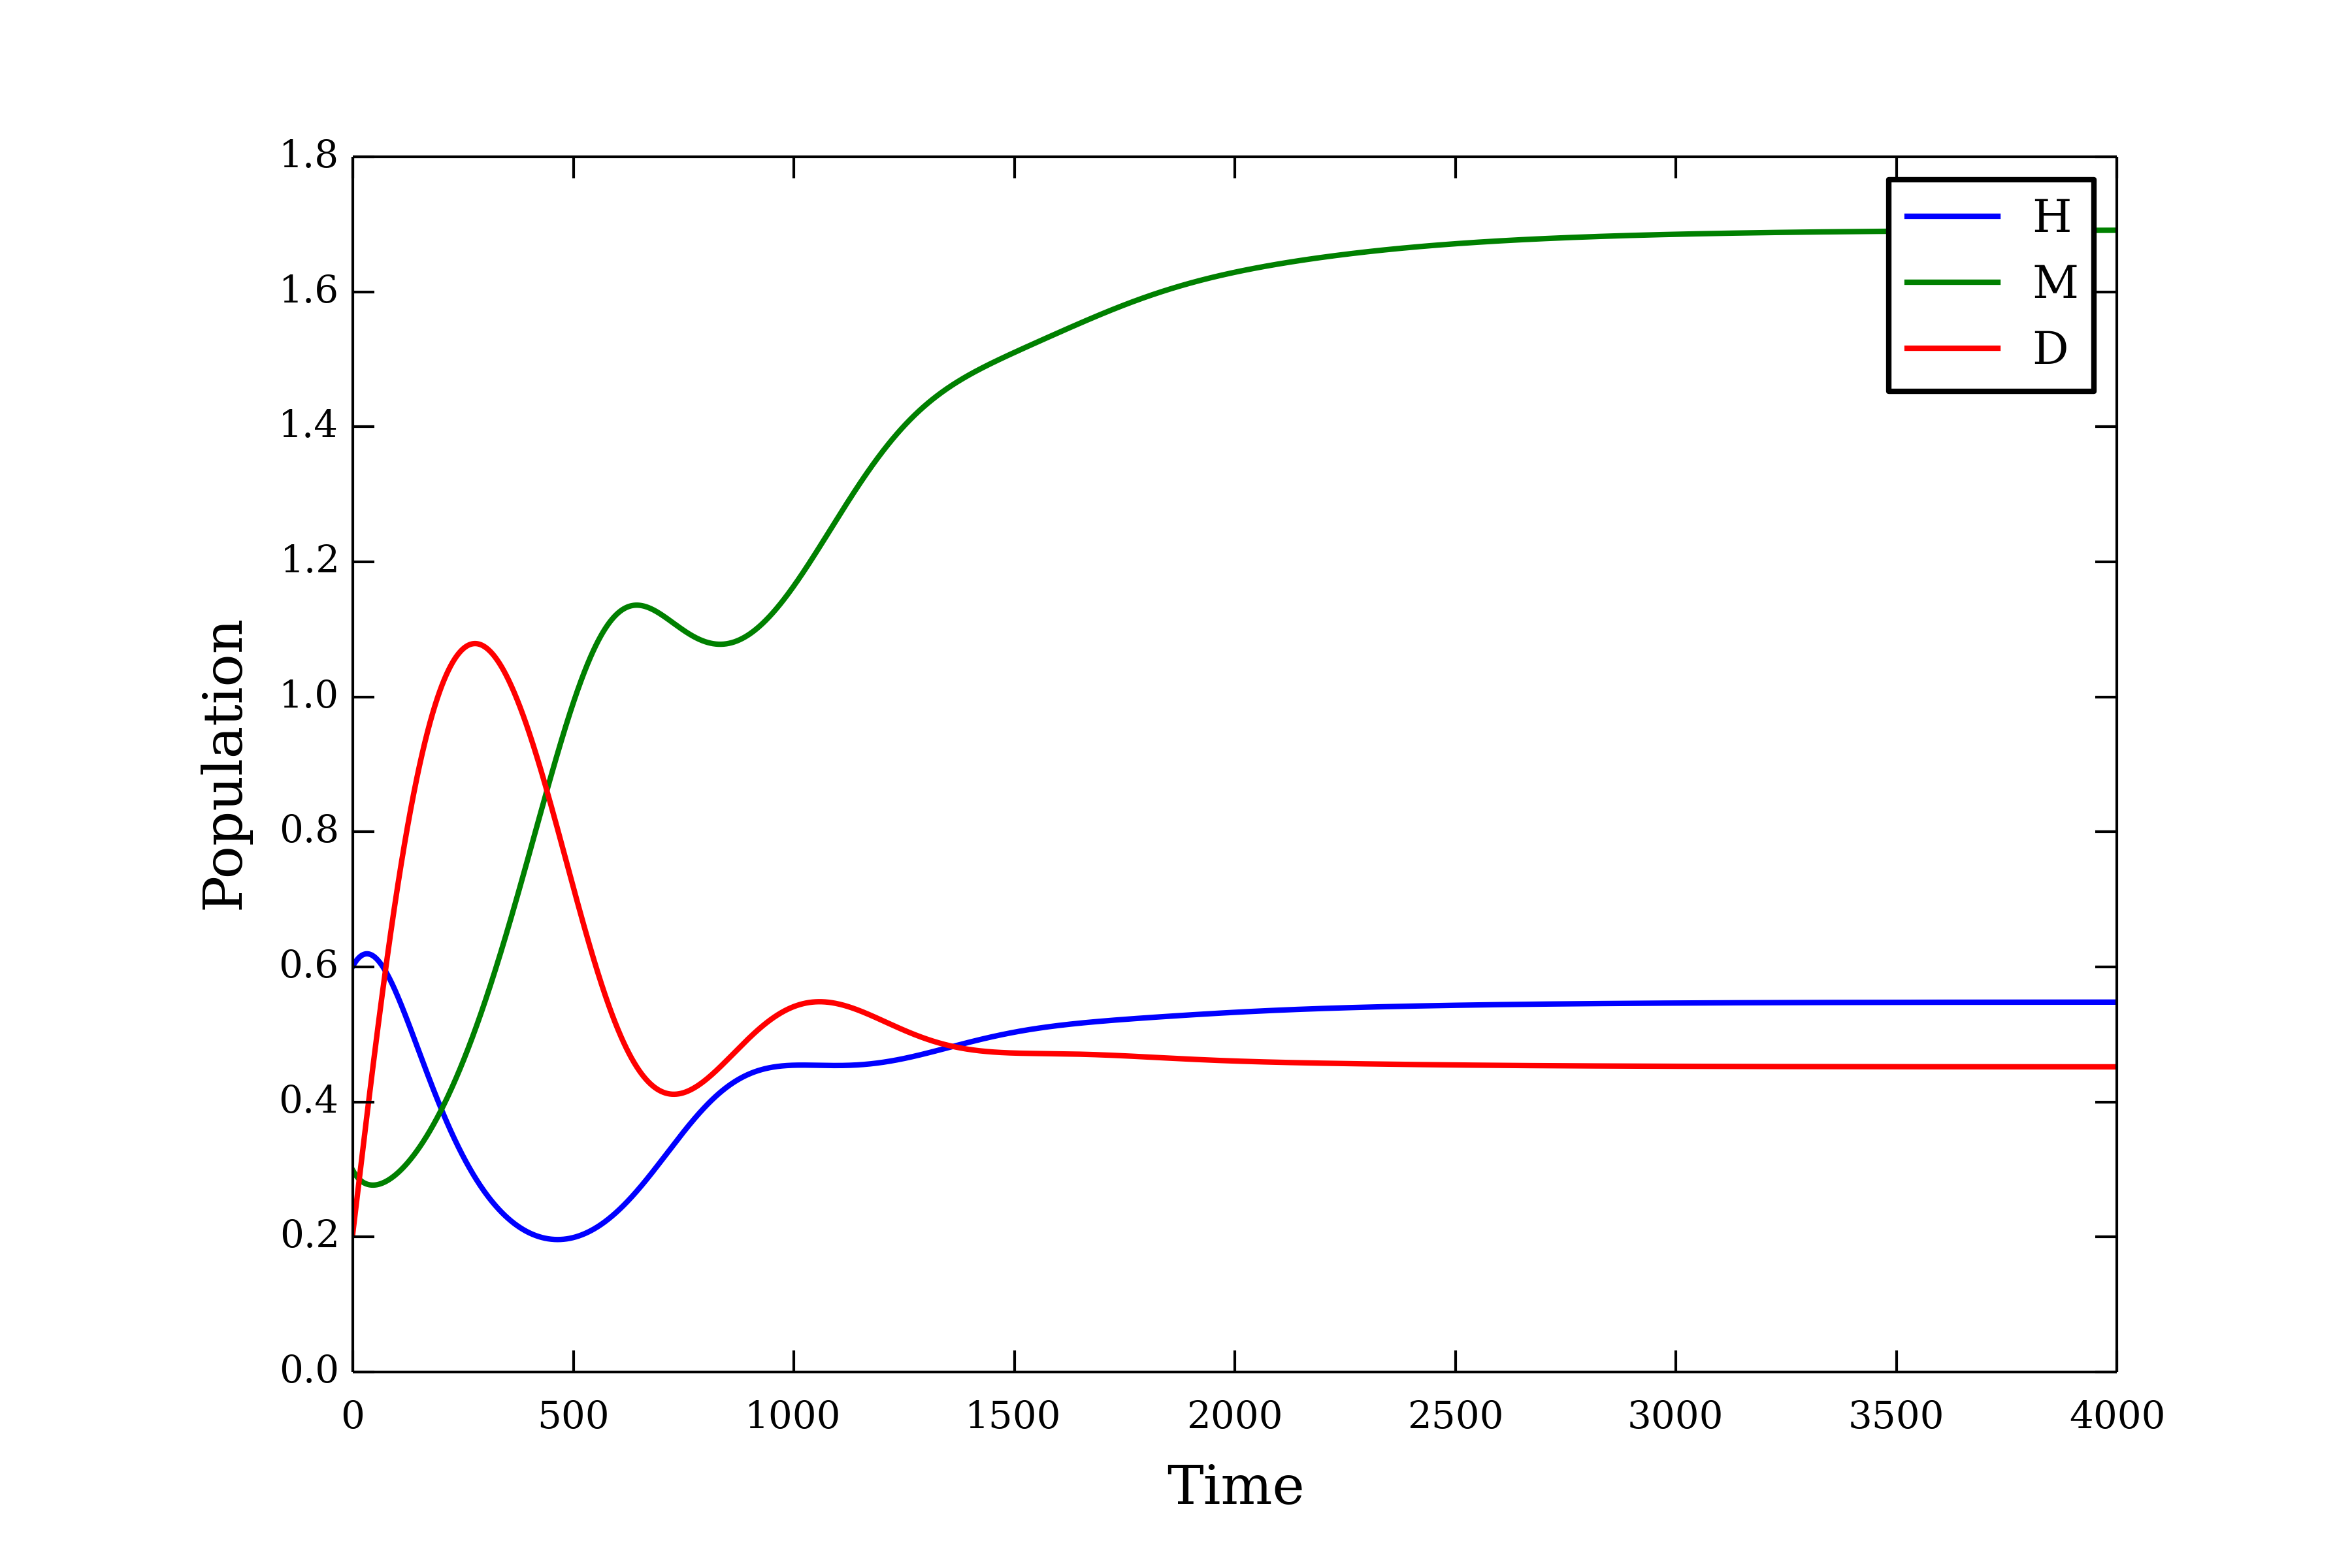
\includegraphics[width=1\textwidth]{equ.png}
\end{frame}

\begin{frame}{Model outcomes: mutant does not invade}
    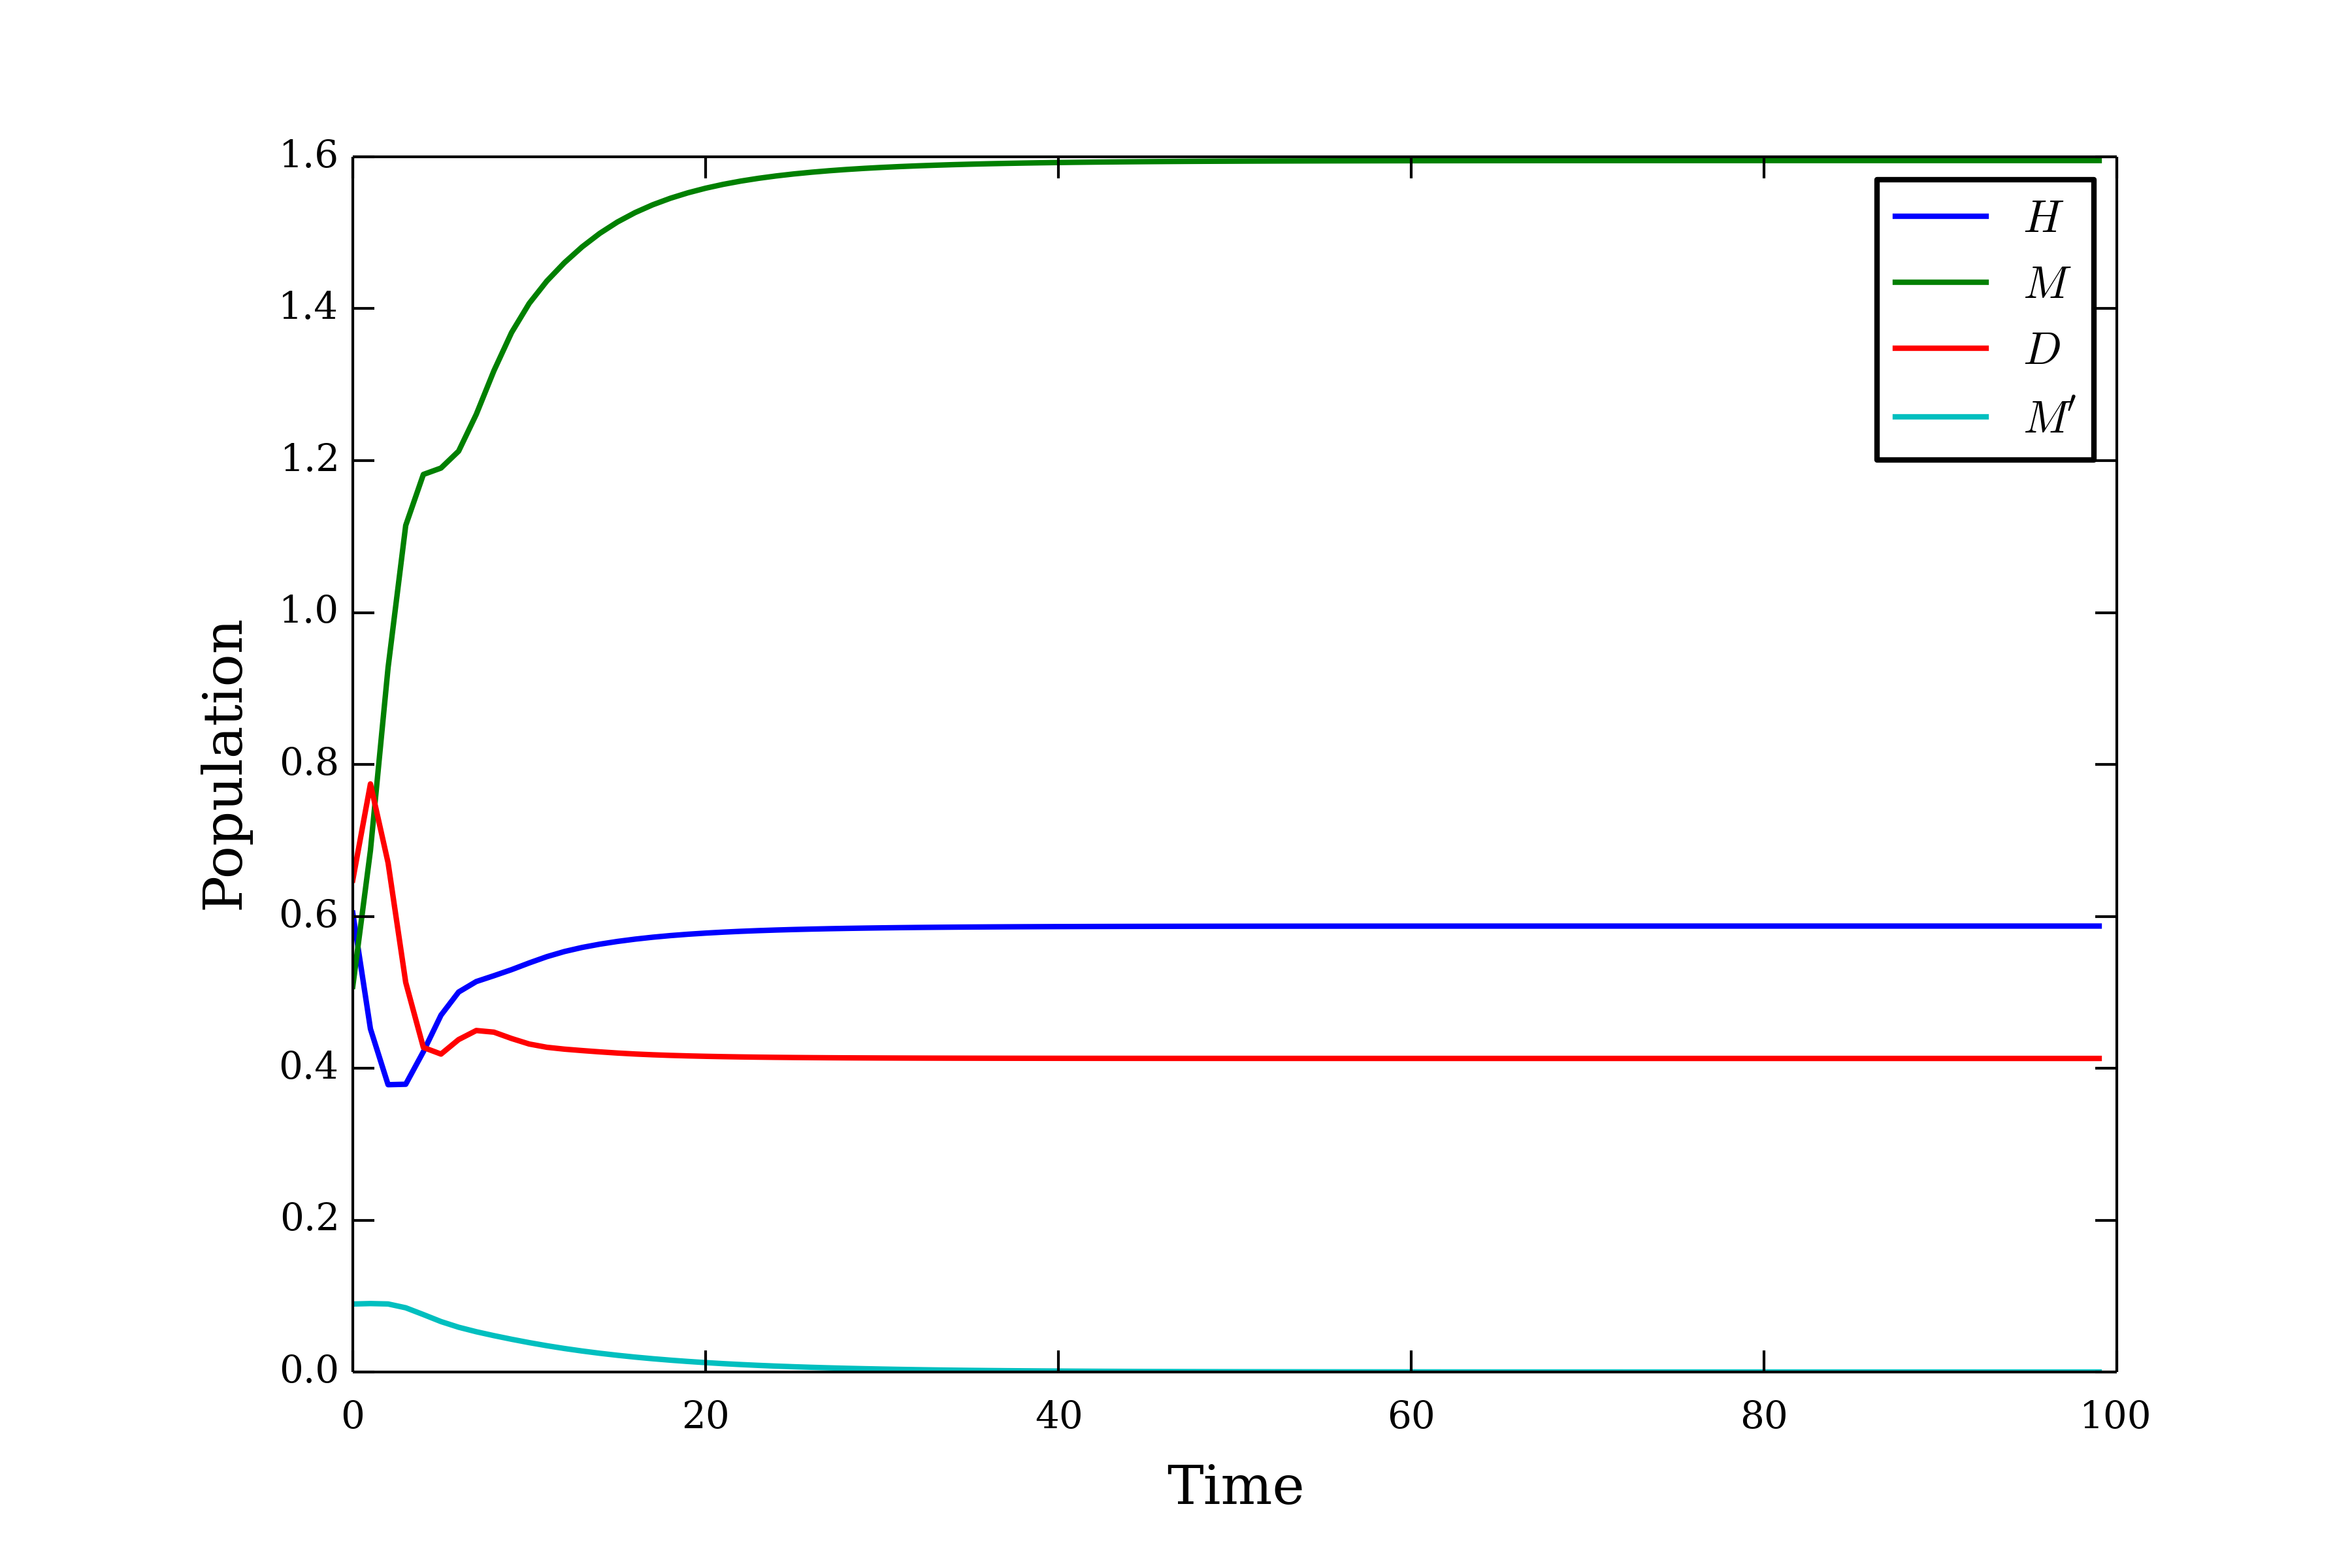
\includegraphics[width=1\textwidth]{dieout.png}
\end{frame}

\begin{frame}{Model outcomes: mutant replaces resident}
    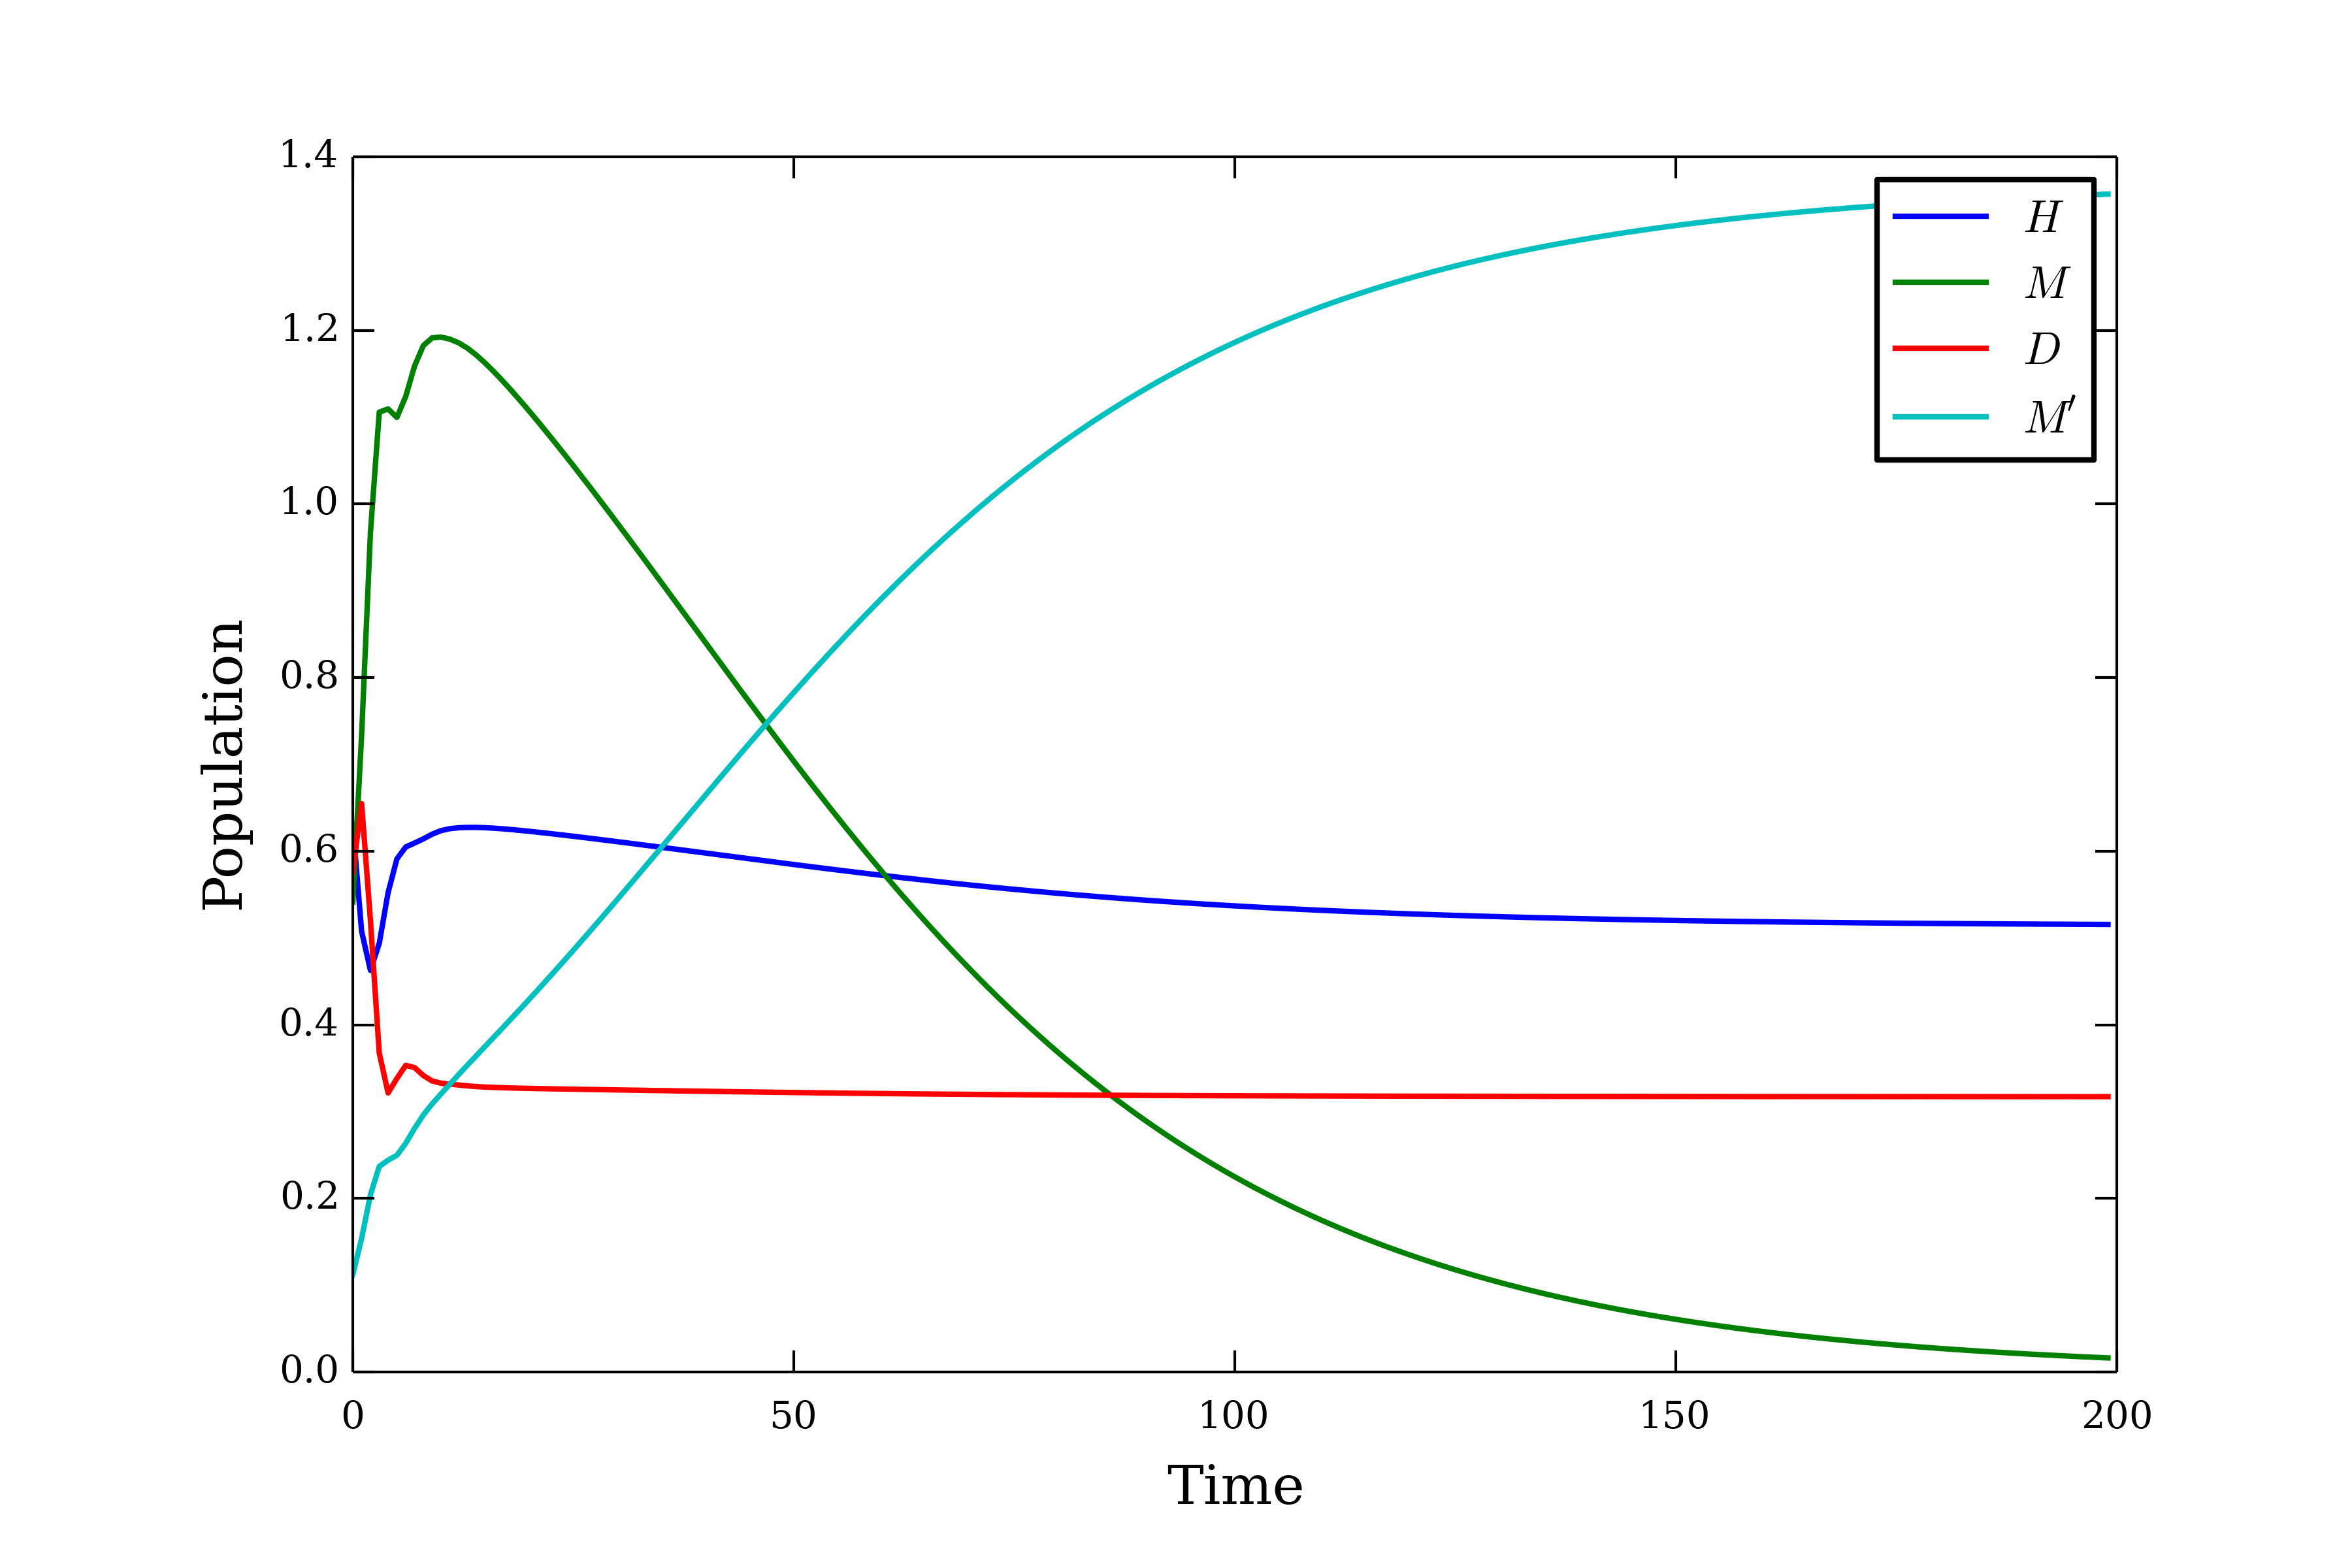
\includegraphics[width=1\textwidth]{replace.png}
\end{frame}

\begin{frame}{Model outcomes: coexistence!}
    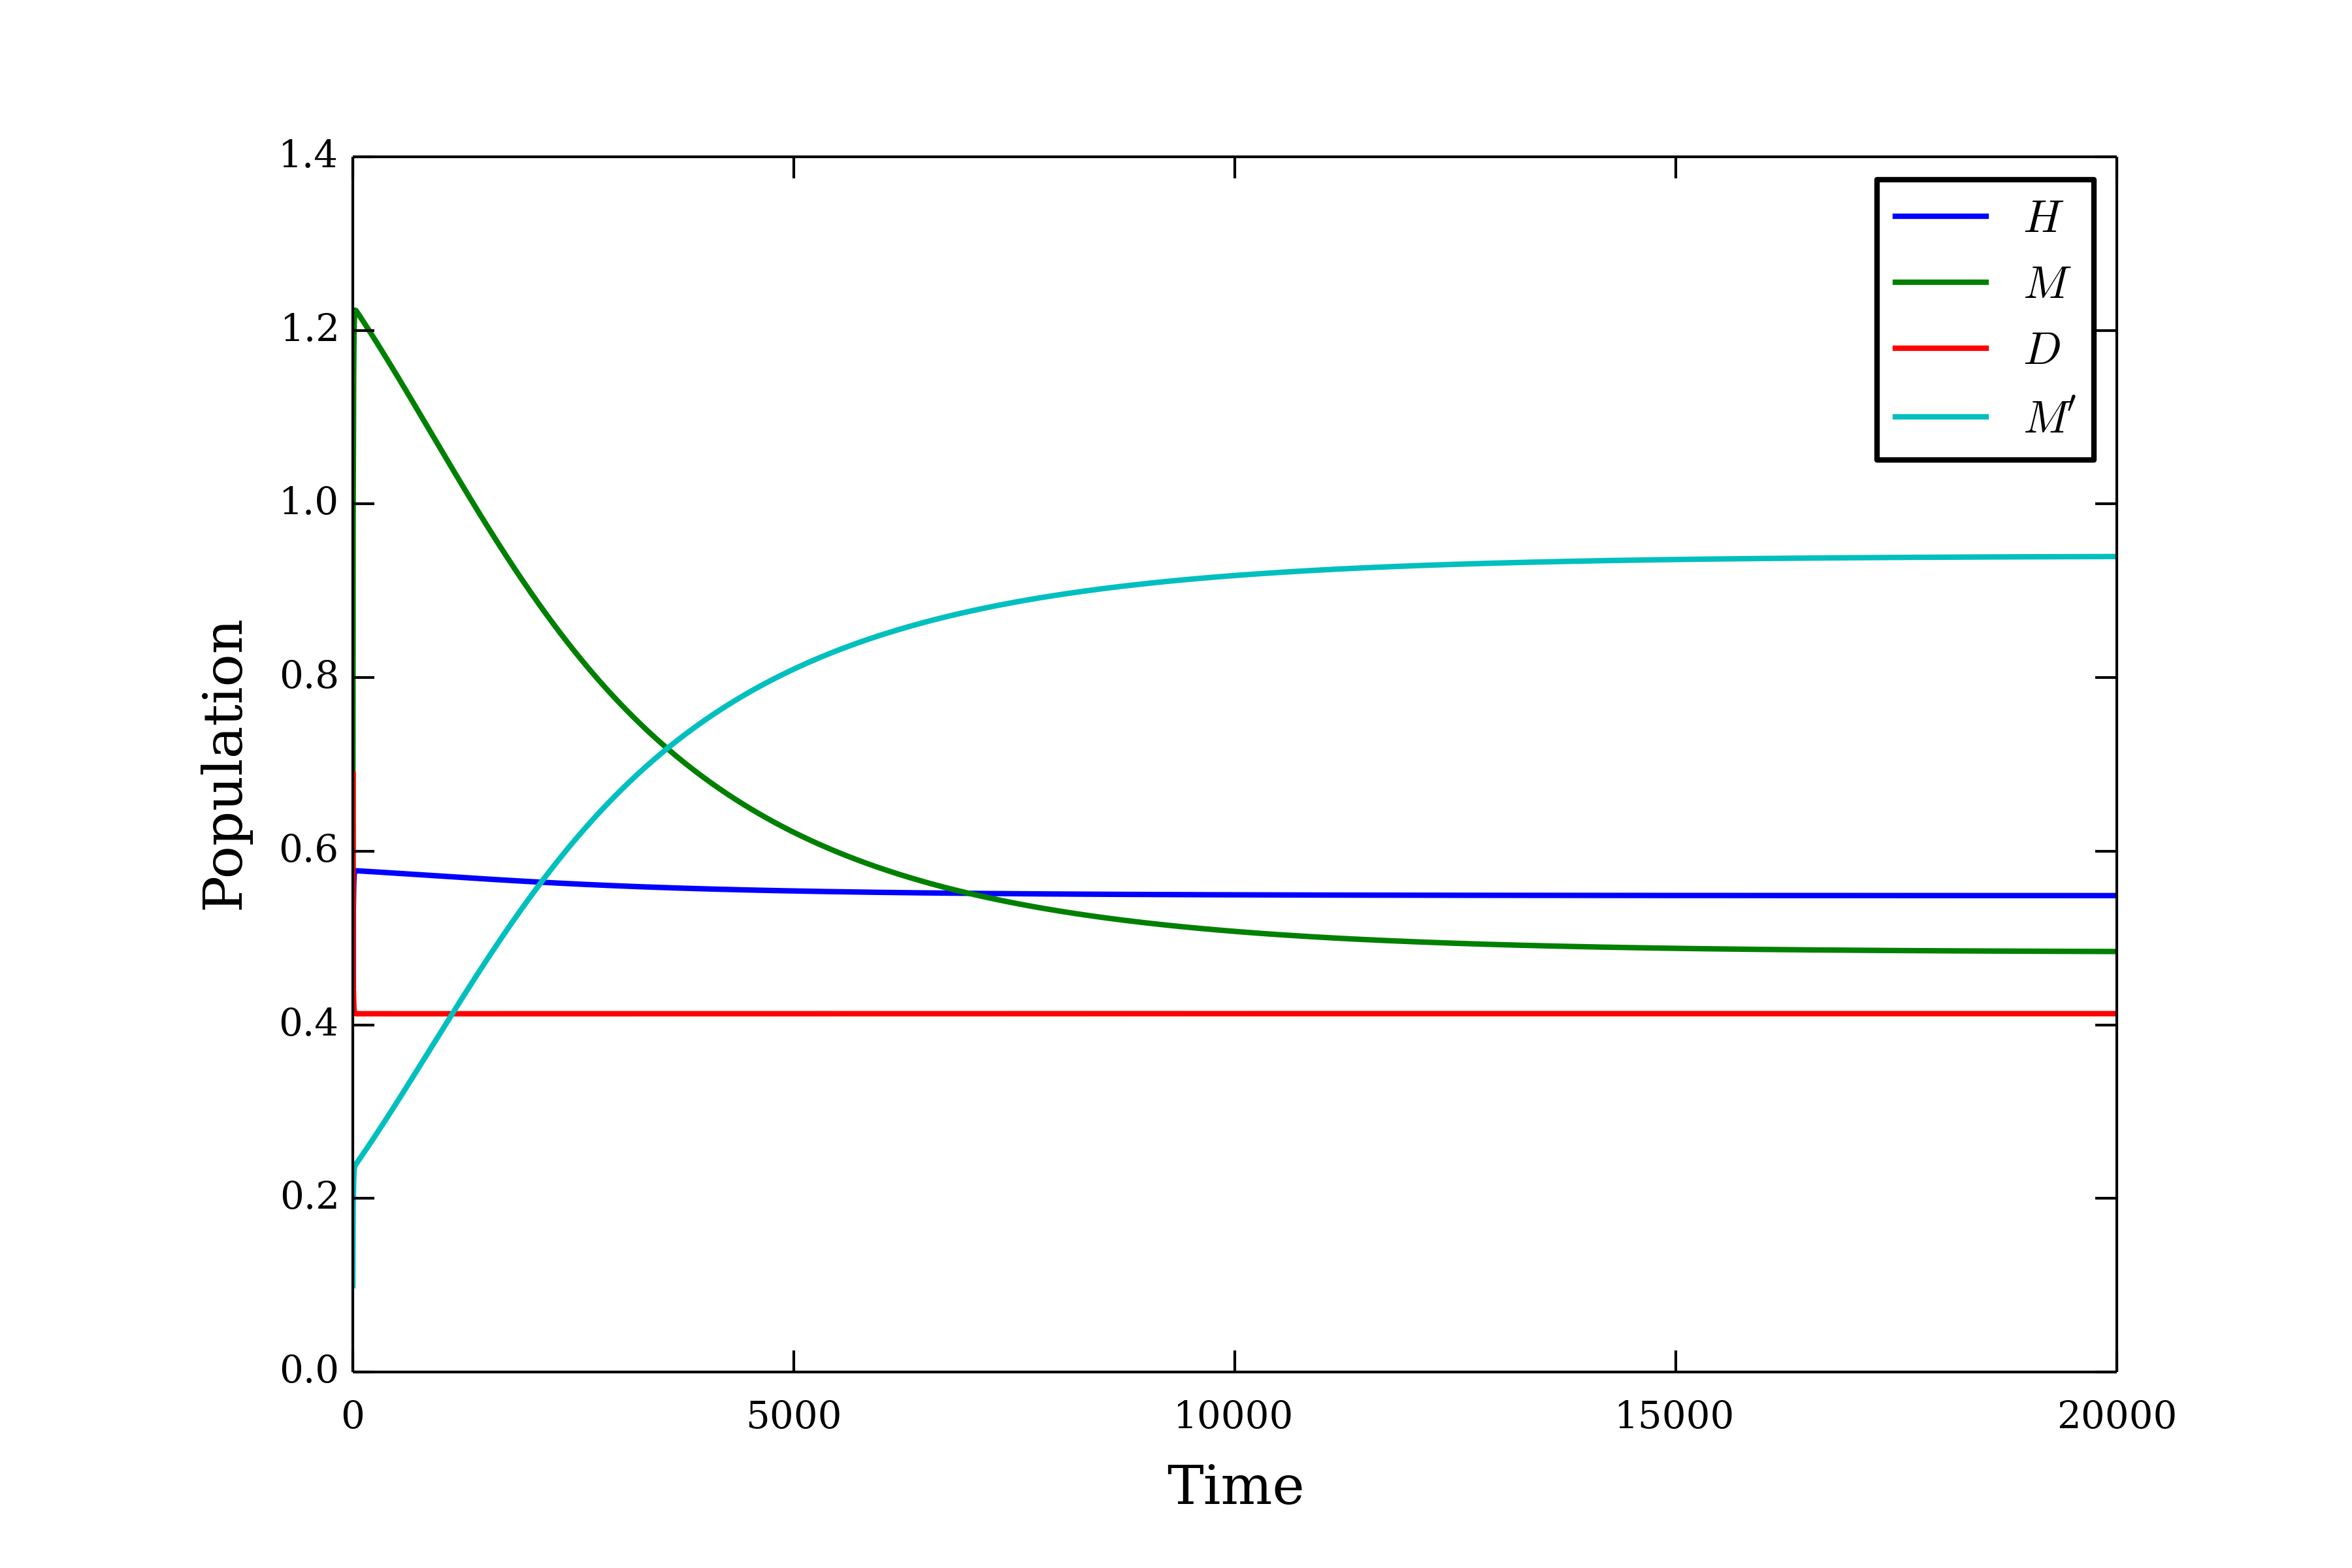
\includegraphics[width=1\textwidth]{coexist.png}
\end{frame}

\begin{frame}{Further work}
    \begin{itemize}
    \item    A more thorough analysis of the model is needed to settle the questions
    posed. 
    
\item A simple invasibility analysis may not suffice
    when there is coexistence between distinct cleaner types.

\item Beyond the initial questions, it would be of interest to assess how the effect of detritus on hosts
    (parameterized by $\alpha$) and environmental conditions (such as host
        growth rate $r$, or detritus decay rate $s$) affect the ESS (if it exists).
    \end{itemize}
\end{frame}

\begin{frame}{}
    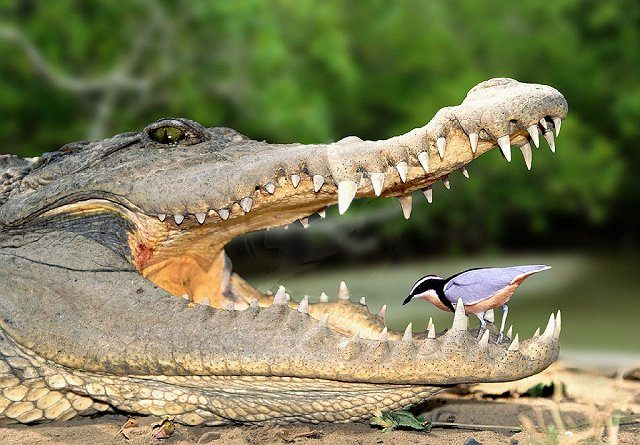
\includegraphics[width=.6\textwidth]{crocodile.jpg} \\[4ex]
    \begin{flushright}
    Thanks for your attention!
\end{flushright}
\end{frame}
\end{document}
